\section*{Divide y vencerás}
    El nacimiento de esta frase se remonta al gran Julio César, prestigioso militar y político romano nacido en los años 100 a.C., teniendo su origen en el hecho de que los romanos al conquistar un territorio, se abstenían de oprimir a los vencidos, evitando rebeliones y la formación de un frente común. Para evitar esto, además los romanos firmaban contratos con cada pueblo de manera individual, otorgando derechos distintos y de número irregular a cada uno, provocando envidias entre los mismos pueblos, y por consiguiente imposibilitando la unión.\\
    
    Con el pasar del tiempo, se convirtió en un refrán popular que implica resolver un problema difícil, dividíendolo en partes más simples tantas veces como sea necesario, hasta que la solución de las partes sea obvia, de esta forma la solución del problema principal se construye con las soluciones encontradas.\\
    
    De esta forma llegó hasta las ciencias de la computación, convirtiéndose en uno de los paradigmas más importantes en el diseño algorítmico. Esta basado en la resolución recursiva de un problema que se divide un subproblemas del mismo tipo hasta que resulten lo suficientemente sencillos para realizar de forma directa. El resultado final entonces, se conforma de la combinación  de los resultados de los subproblemas, dando una solución final al problema general.\\
    
    De esta técnica se tienen algoritmos muy eficientes para la resolución de cualquier tipo de problema, ejemplos basados en esta técnica se tiene:\\
    \begin{itemize}
        \item Algoritmo de Ordenamiento: QuickSort, MergeSort
        \item Multiplicar números grandes: Karatsuba
        \item Análisis sintáctico: análisis sintáctico top-down
        \item Transformada discreta de Fourier
    \end{itemize}
    
\section*{Algoritmos de ordenamiento}
    Los algoritmos de ordenamiento son algoritmos que colocan los elementos de un array, lista o vector, en una secuencia específica descrita por una relación de orden.\\
    
    Los órdenes más comunes son el numérico y lexicográfico, siendo el último una relación de orden definida sobre el producto cartesiano de conjuntos ordenados. Es principalmente concido por la aplicación a cadenas de caracteres en diccionarios, guias telefónicas, etc.\\
    
    La salida de estos algoritmos deben de satisfacer 2 condiciones:
    \begin{enumerate}
        \item La salida debe de encontrarse en orden no-decreciente
        \item La salida es una permutación o re-ordenamiento de la entrada
    \end{enumerate}
    
    Hay métodos muy simples de implementar que son útiles en los casos en dónde el número de elementos a ordenar no es muy grande. Pero por otro lado hay métodos sofisticados, más difíciles de implementar pero que son más eficientes en cuestión de tiempo de ejecución.
    
    Los métodos sencillos por lo general requieren de aproximadamente n x n pasos para ordenar n elementos.
    
    Los métodos simples con complejidad cuadrática son:
    \begin{itemize}
        \item Insertion Sort
        \item Selection Sort
        \item Bubble Sort
        \item Shell Sort(extensión más veloz del bubble sort)
    \end{itemize}
    
    Los métodos más complejos acortan el tiempo de ejecución y por lo tanto son más eficiente:
    \begin{itemize}
        \item Quick Sort
        \item Merge Sort
        \item Heap Sort
        \item Radix
        \item Address-calculation Sort
    \end{itemize}
    
    Existen diferentes maneras de clasificar los algoritmos de ordenamiento:
    
    \textbf{Clasificación según el lugar donde se realiza la ordenación}\\
    \begin{itemize}
        \item Ordenamiento interno: Se realiza el ordenamiento enteramente en la memoria primaria del ordenador
        \item Ordenamiento externo: Aquellos que involucran discos auxiliares para guardar resultados intermedios
    \end{itemize}
    
    \textbf{Clasificación por el tiempo que tardan en la ordenación}\\
    \begin{itemize}
        \item Ordenación natural: Tarda lo mínimo posible con la entrada ordenada
        \item Ordenación no natural: Tarda lo mínimo posible cuando la entrada esta inversamente ordenada 
    \end{itemize}
    
    \textbf{Por estabilidad}\\
    En un ordenamiento estable se mantiene el orden relativo que tenian originalmente los elementos con claves iguales. Esto es, con un algoritmo estable habrá 2 registros R y S con la misma clave y con R apareciendo antes que S en la lista original.\\
    
    En elementos que son indistiguibles entre si, la estabilidad no es un problema, tal y como sucede con los números enteros, pero en general se puede decir que se despecia la estabilidad cuando el elemento entero es la clave.\\
    
\section*{Merge Sort}
    Merge Sort es un algoritmo desarrollado con la técnica de divide y vencerás, creado por Jhon Von Newmann en 1945. De propósito general, es un algoritmo que produce un ordenamiento estable con complejidad O(nlogn). Utiliza memoria auxiliar con complejidad O(n), dado por el algoritmo \textit{Merge}.\\
    
    La familia de algoritmos \textit{Merge}, toman una multiple lista ordenada como entrada y produce una lista única ordenada como salida, conteniendo todos los elementos de la lista de entrada. Estos algoritmos son utilizados como subrutinas para varios algoritmos de ordenamiento, siendo el más famoso precisamente \textit{Merge Sort}.\\
    
    \textit{Merge Sort} inicia con la entrada de un arreglo, este divide el arreglo de entrada en 2 mitades, se llama a si mismo para las 2 mitades y después mezcla las mitades con ayuda del algoritmo \textit{Merge}.\\
    
    Gráficamente la operación del algoritmo se muestra en la siguiente figura \ref{OperacionMergeSort}:
    \begin{figure}[h!]
        \centering
        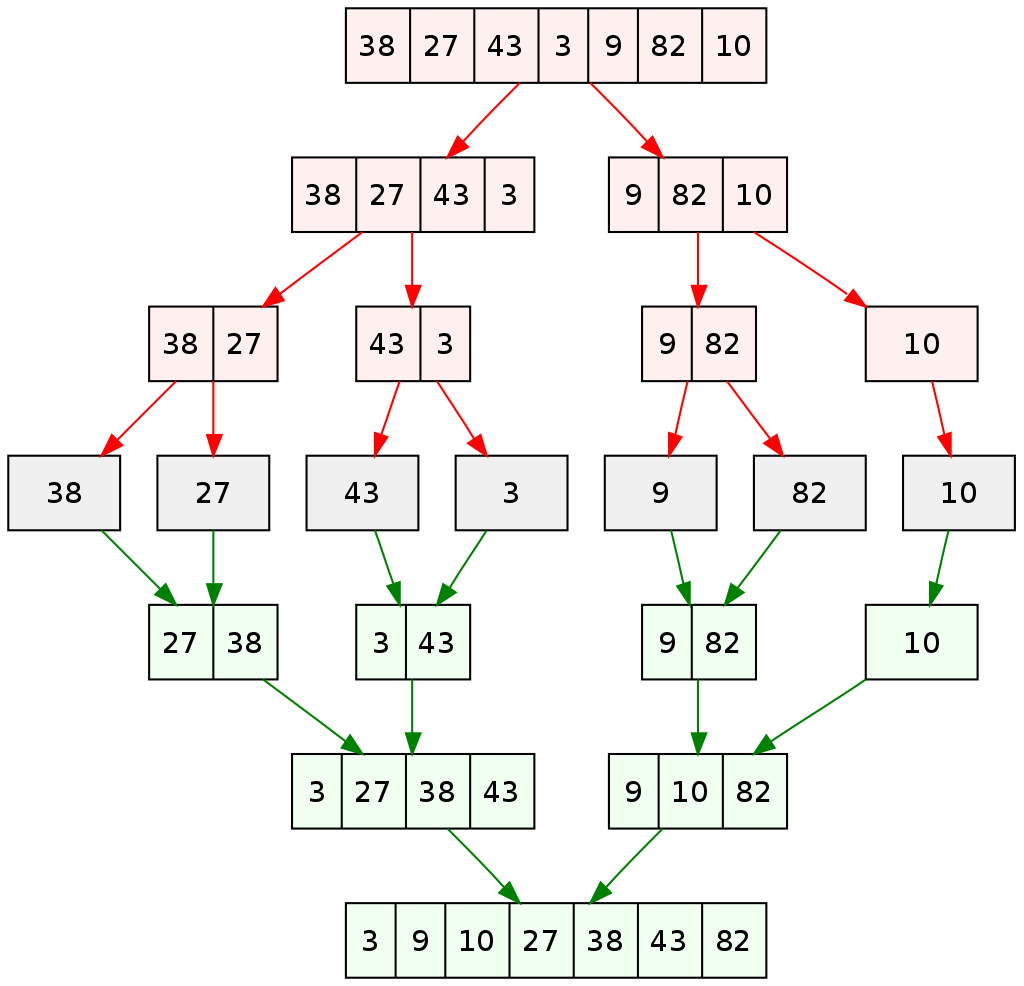
\includegraphics[width=10cm]{OperacionMergeSort.png}
        \caption{Ordenamiento de un arreglo de 7 valores enteros utilizando el algoritmo \textit{MergeSort}}
        \label{OperacionMergeSort}
    \end{figure}
    
\section*{Quick Sort}
    Quick Sort es un algoritmo basado en la técnica divide y vencerás creado por el científico británico C. A. R. Hoare, quién también es conocido como Tony Hoare, en el año de 1960.\\
    
    Es el algoritmo más ampliamente utilizado en el mundo para el ordenamiento numérico, también es considerado el algoritmo más eficiente y veloz de los métodos de ordenación interna.
    
    La complejidad del algoritmo para su caso promedio es O(nlogn), pero en su peor caso tendrá la complejidad O($n^2$), dandose este caso cuando el pivote queda en alguno de los extremos.
    
    El funcionamiento del algoritmo se describe en 4 pasos:\\
    \begin{enumerate}
        \item Se elige un elemento de la lista a ordenar, se le llamará pivote
        \item Se reacomodan los elementos de la lista según el valor de pivote, de manera que los elementos antes de este son siempre menores, y los que están después serán siempre mayores. Después de este ordenamiento parcial, el pivote ya se encuentra colocado en el lugar exacto que debe ocupar en la lista final.
        \item La lista se separa en 2 sublistas, una formada por los elementos a la izquierda del pivote, y otra por los elementos a su derecha.
        \item Se repite el proceso de forma recursiva para todas las sublistas mientras estas contengan más de un elemento. Al terminar este proceso todos los elemento se encuentran ordenados.
    \end{enumerate}
    
    En este algoritmo la elección del pivote es muy importante, pues dependiendo de la elección, el algoritmo puede ser más o menos eficiente. Si bien tomar un elemento cualquiera como pivote no requiere de cálculo alguno, la elección a ciegas puede provocar para ciertas entradas una complejidad de O($n^2$).\\
    
    Una alternativa para subsanar este problema es conocer de antemano el elemento central para utilizar como pivote, esta operación puede realizarse en O(n) y asegura hasta para el peor de los casos que el algoritmo sea O(nlogn), sin embargo este cálculo adicional rebaja la eficiencia en el caso promedio.\\
    
    Otra opción es tomar tres elementos de la lista, comúnmente se escoge el primero, medio y último elemento del arreglo, se comparan y el valor medio es escogido como el pivote.